\subsubsection{Каскад ОК}

\begin{center}
\begin{figure}[h!]
\center{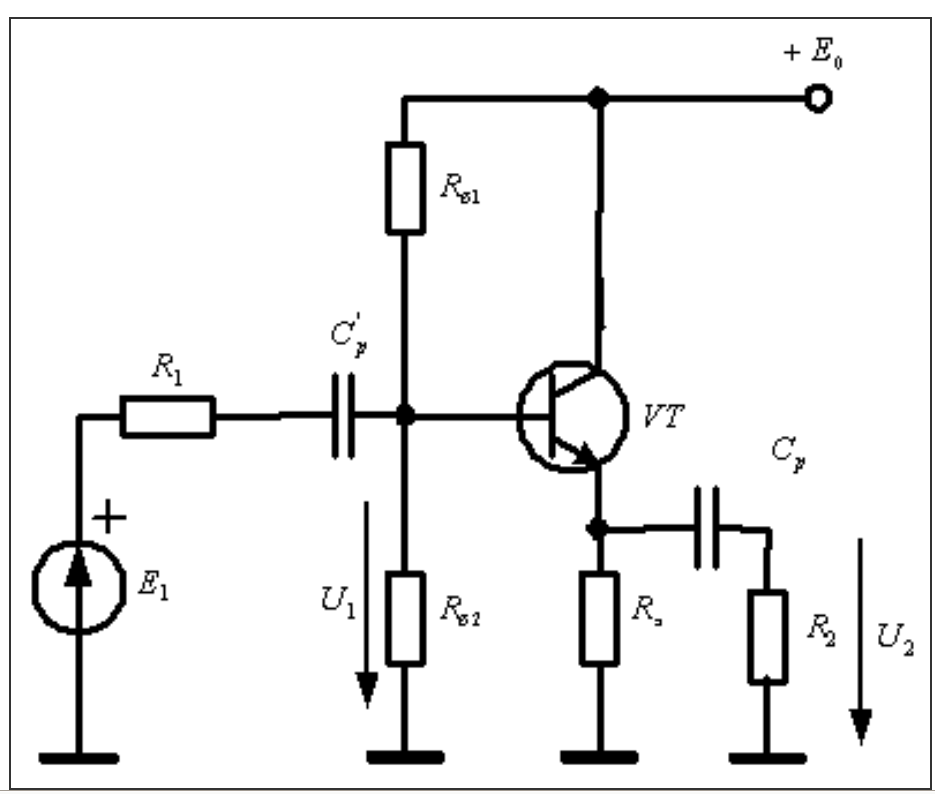
\includegraphics[scale=0.45]{OK.png}}
\caption{ОК}
\end{figure}
\end{center}

\begin{center}
\begin{figure}[h!]
\center{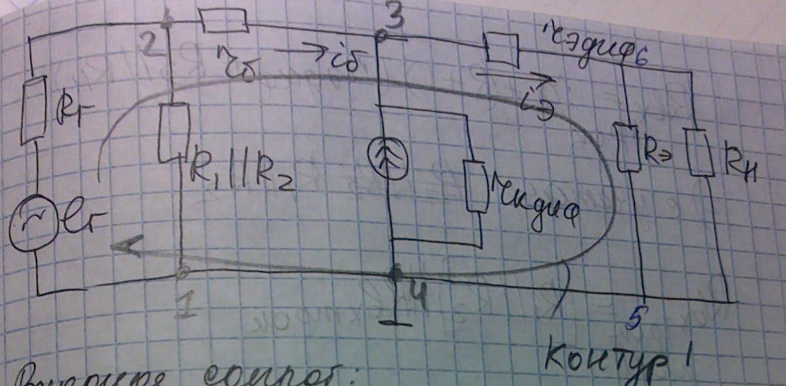
\includegraphics[scale=0.7]{OK1.png}}
\caption{ОК1}
\end{figure}
\end{center}

Важные моменты:
1) Нагрузка цепляется в цепь Э, следовательно 100$\%$ отрицательная связь;
2) Большое входное сопротивление;
3) Малое выходное (хорошее согласование);
4) Не усиливает по напряжению, лучше всех усиливает по току.

1. Входное сопротивление:
$$
R_{in} = \frac{U_{in}}{I_{in}}
$$

$$
U_{in} = e_{g}-i_{in}*R_g
$$
1) Без учёта $R_{1}||R_{2}$:
Контур 1-2 по второму закону Кирхгофа:
$$
U_{in}=\varphi_2 - \varphi_1 = i_br_b + i_e(R_e||R_{out}) + r_{e_{dif}}) = i_{b}(r_{b} + (B+1)(R_{e}||R_{out}+r_{e_{dif}}))
$$

$$
R_{in}=\frac{U_{in}}{i_{in}}=\frac{i_{b}(r_{b} + (B+1)*(R_{e}||R_{н}+r_{e_{dif}}))}{i_{b}}
$$

$$
R_{in_{trOK}}= r_{b} + (B+1)*(r_{e_{dif}}+R_{e}||R_{out})
$$

2) С учётом $R_{1}||R_{2}$:

$$
R_{in_{trOK_{full}}}= [R_{1}||R_{2}]||R_{in_{trOK}}
$$

2. Выходное сопротивление:
Выходное сопротивление определяется при отключенном напряжении и при нулевом (?) входном сигнале:
$$
R_{out}=\frac{U_{xx}}{I_{kz}}
$$

$$
U_{xx}=U_{56}(R_{out}=0) wtf!!
$$

Контур 1: клеммы на нагрузке замкнуты: $ I_{kz}=I_{e} $
$$
U_{56}=U_{R_{1}||R_{2}}+U_{r_{b}}+U_{r_{e_{dif}}} = \left[ \frac{R_{1}||R_{2}+r_{b}}{B+1}+r_{e}\right ]i_{e}
$$
$$
R_{\Sigma_{56}}=\left[\left(\frac{R_{1}||R_{2} + r_{b}}{B+1} + r_{e}\right) || R_{e}\right]
$$
$$
U_{xx}=R_{\Sigma_{56}}i_{e}
$$
$$
R_{out}=\frac{R_{\Sigma_{56}}*i_{e}}{i_{e}}=R_{\Sigma_{56}}=[\frac{R_{1}||R_{2} + r_{b}}{B+1}+r_{e}]||R_{e}
$$
3. Коэффициент передачи по напряжению:
$$
K_{U_{OK}}= \frac{U_{out}}{U_{in}} = \frac{i_e(R_{e}||R_{out})}{\Delta*(R_{in_{trOK}})}
$$
4. Коэффициент передачи по току:
$$
K_{I_{OK}}= \frac{i_{out}}{i_{in}}
$$
\begin{center}
\begin{figure}[h!]
\center{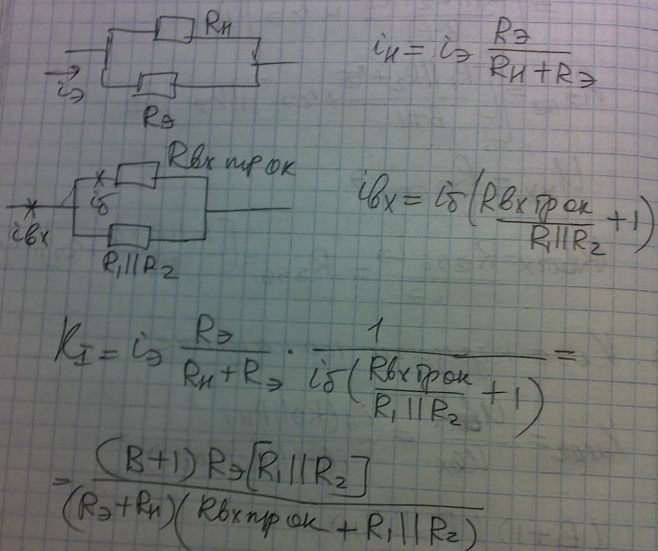
\includegraphics[scale=0.7]{OK2.png}}
\end{figure}
\end{center}

